\section{Results}
    \subsection{Changes in Land Use and Land Cover}
    \subsection{Drought State Transitions}
    	The Table \ref{tb:abs_freq_drought_class}  presents the relative frequency of each meteorological (SPI-12) and hydrological (SRI-12) drought class for the periods P1 and P2. In P1 period, it can be observed that the most recurrent drought classes are ND and mD for both SPI-12 and SRI-12. Between periods P1 and P2, similar changes in relative frequencies are observed for both drought indexes, they are: reductions in the relative frequencies of drought classes ND, mD and MD and an increase in the relative frequency of class SED.
    	
    	In period P2, the drought class ND remains the one with the highest relative frequency for both SPI-12 and SRI-12. For SPI-12, there is an increase of 11.44\% in the relative frequency of the SED class and a decrease of 8.56\% in the mD class between P1 and P2, equalizing the relative frequency of these two classes in P2. For SRI-12, the changes in relative frequencies for SED and mD classes between P1 and P2 periods are, respectively, $+14.67\%$ and $-8.22\%$. Despite these changes in relative frequencies, ND and mD classes of SRI-12 are still the most recurrent in the P2 period.
    	 
		\begin{table}[width=.9\linewidth, cols=5]
            \caption{
            Relative Frequencies of SPI and SRI drought classes in P1 (50 yrs) and P2 (36 yrs) periods.
            }
            \label{tb:abs_freq_drought_class}
             \begin{tabular*}{\tblwidth}{@{\extracolsep{\fill}} c| c c c c}
            \toprule
                  & ND & mD & MD & SED & Duration\\
            \midrule
                SPI-12 (P1) & 50.00\% & 28.00\% & 14.00\% & 8.00\% \\
                SPI-12 (P2) & 47.22\% & 19.44\% & 13.89\% & 19.44\% \\
                SRI-12 (P1) & 56.00\% & 36.00\% & 6.00\% & 2.00\% \\
                SRI-12 (P2) & 50.00\% & 27.78\% & 5.56\% & 16.67\% \\
            \bottomrule
            \end{tabular*}
        \end{table}  
  
        The Figure \ref{fig:t_probs} shows the transition matrices of the meteorological and hydrological droughts classes for both P1 and P2 periods.
        
        Regarding the changes in the transition probabilities of hydrological droughts (SRI-12), significant changes can be observed given the occurrence of both SED and MD drought classes. For the occurrence of the SED drought class, the transition probabilities in period P2 are 66.67\% to remain in the SED class and 16.67\% to regress to the MD or md drought classes; in period P1, the unique possible transition, i.e. 100\% probability, is to regress to a MD drought class.

        In relation to MD drought class occurrence, two equiprobable transitions are observed in period P2: progress to SED drought class or regress to mD drought class, and three equiprobable transition are seen in period P1: permanence in the MD drought class or regression to the mD or ND drought classes.

        No significant changes were observed in the transition probabilities given the occurrence of the ND or mD classes, however, the possibilities of transition from ND to SED (3.7\%) in the P1 period, which does not occur in the P2 period, and transition from mD to SED (11.11\%) in the P2 period, that does not occur in the P1 period, can be highlighted.

        Concerning the changes in the transition probabilities of meteorological droughts (SPI-12), except for the occurrence of the mD class, no changes were observed in the possible transitions, only in the values of the transition probabilities. 
        
        For an occurrence of mD drought class, one can observe that there are three possibles transitions in P1 period are: regress to ND (35.71\%), permanence in mD class (42.86\%) and progress to MD class (21.43\%). However, in P2 period, these three possibles transition are reduced from two: regress to ND (71.43\%) and progress to SED (28.57\%).

        It is worth noting the changes in the probabilities of the possible transitions between the P1 and P2 periods, given the occurrence of a ND drought class. In P1 period, the most probable transition for this drought class occurrence is to remain in the ND class (52.00\%). In P2 period, two equiprobable transitions appear: permanence in ND class (31.25\%) and progress to SED class (31.25\%). An increase in the probability of progression for MD can also be observed from 12.0\% at P1 to 25.0\% at P2
        
        \begin{figure*}
            \centering
                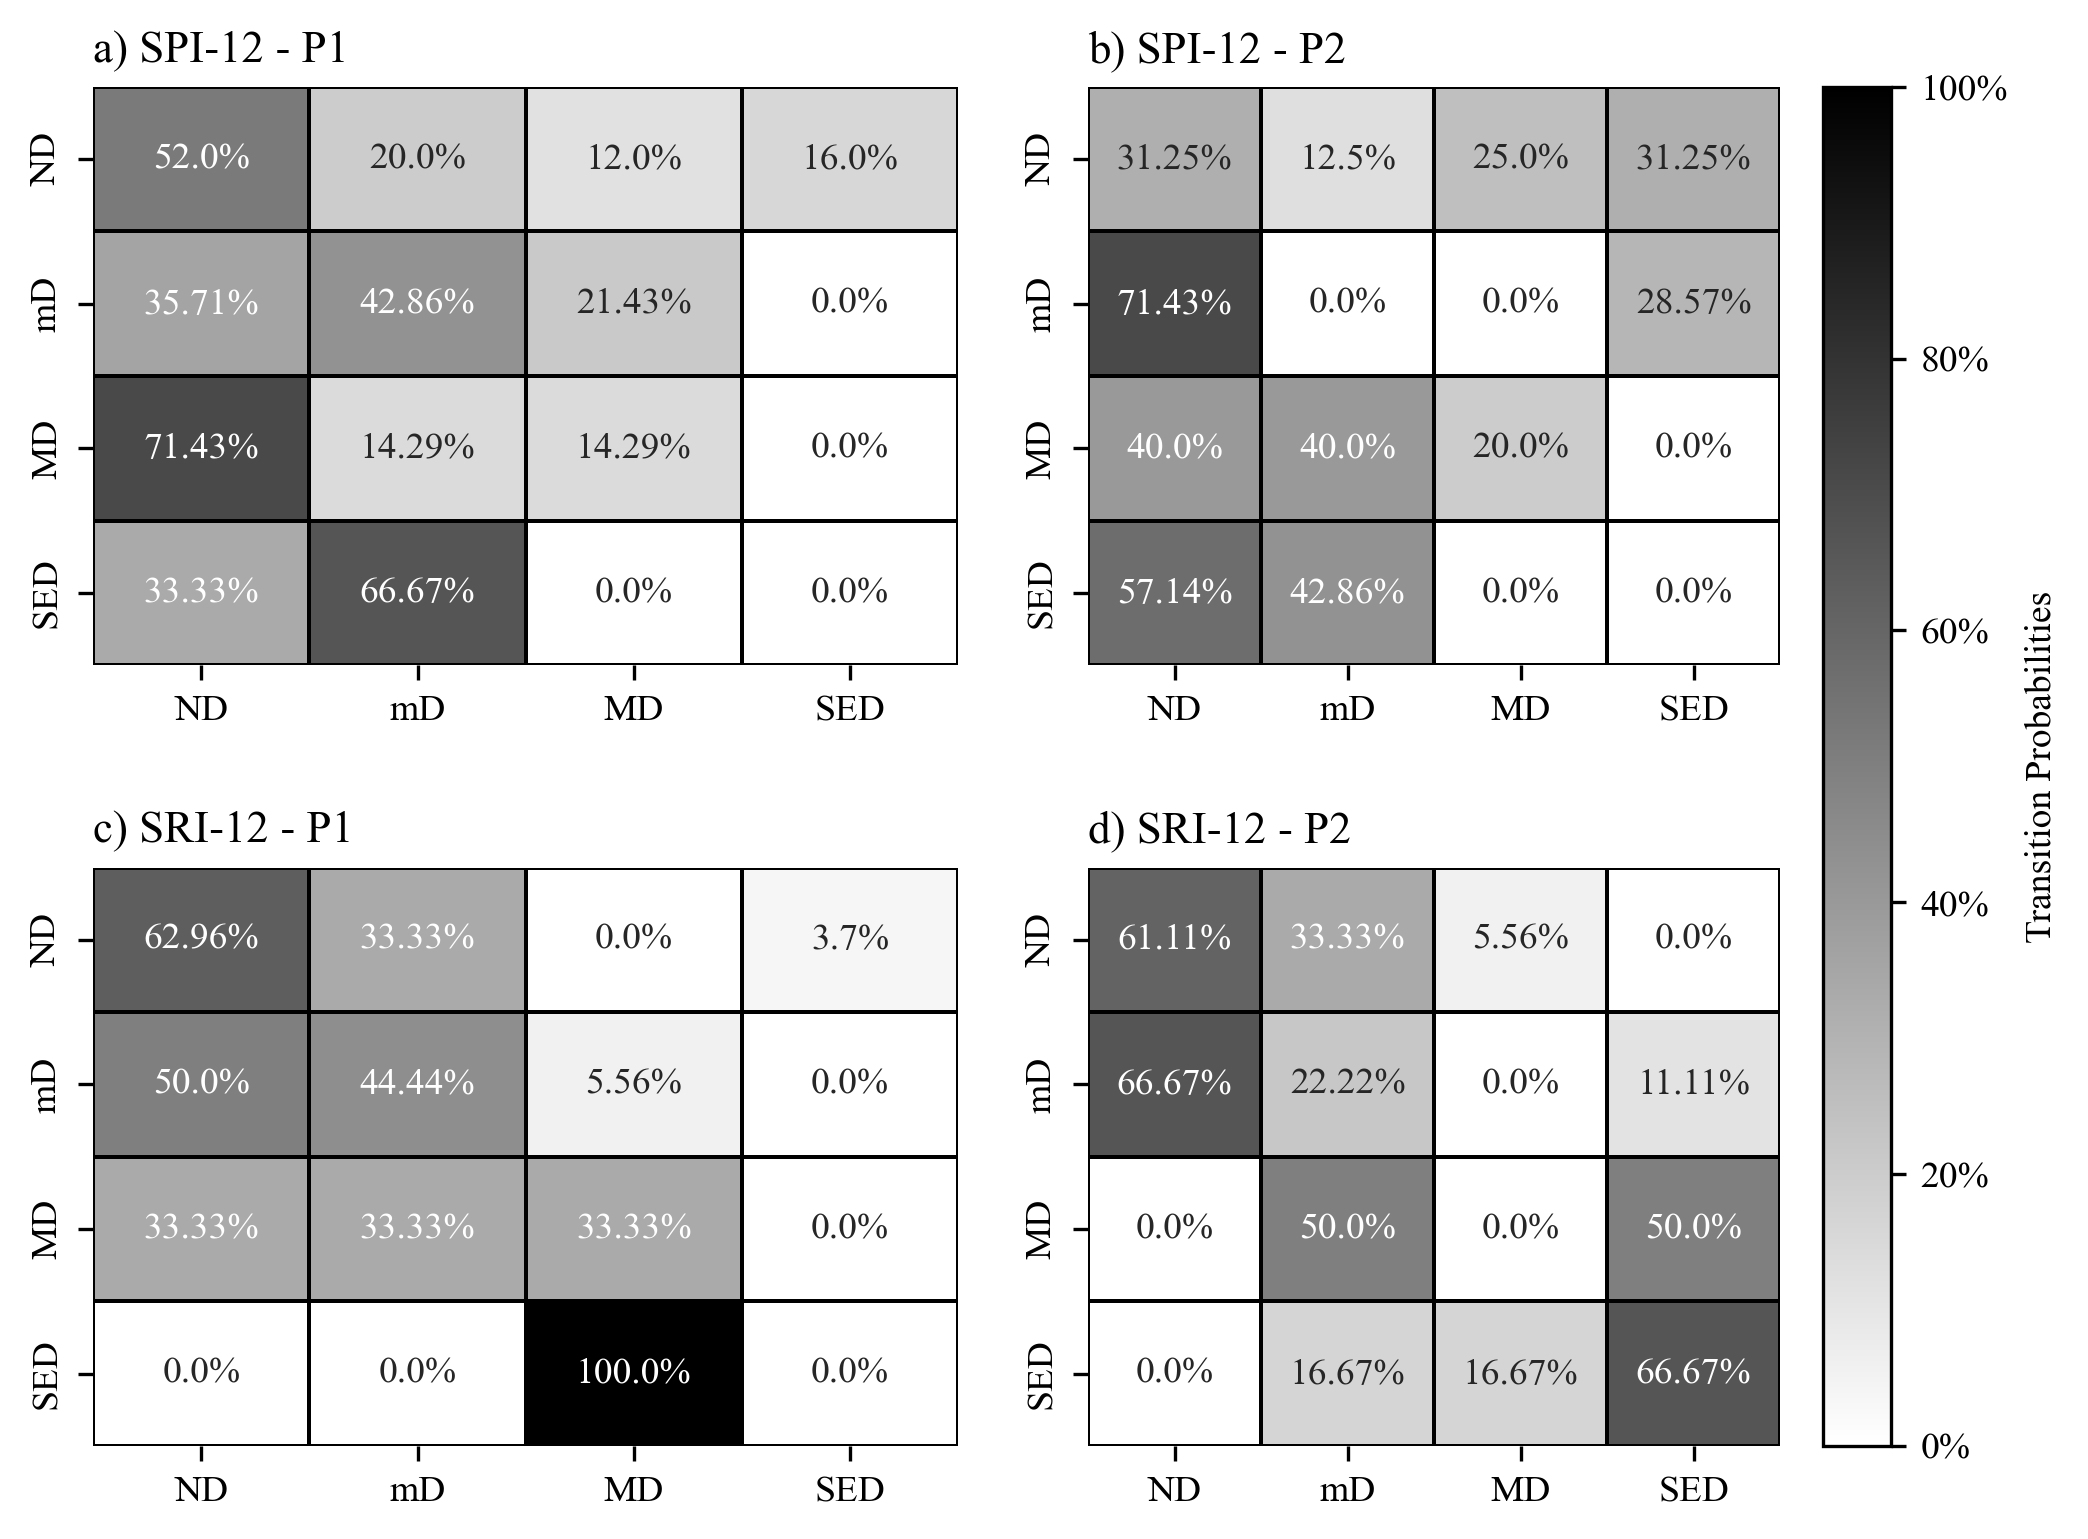
\includegraphics[scale = 1]{
                figs/SPI_SRI_Transition_Matrix.png
                }
            \caption{
                Transition matrices of the adopted drought classes for the following time series: a) SPI-12 in period P1, b) SPI-12 in period P2, c) SRI-12 in period P1 and d) SRI-12 in period P2
            }
            \label{fig:t_probs}
        \end{figure*}
        
        \begin{table}[width=.9\linewidth, cols=5]
            \caption{
            Stationary distribution of the Markov chains constructed for SPI-12 and SRI-12 for both P1 and P2 periods.
            }
            \label{tb:std_distr}
            \begin{tabular*}{\tblwidth}{@{\extracolsep{\fill}} c| c c c c}
            \toprule
                  & ND & mD & MD & SED\\
            \midrule
                SPI-12 (P1) & 48.49\% & 29.57\% & 14.18\% & 7.76\% \\
                SPI-12 (P2) & 45.71\% & 20.00\% & 14.29\% & 20.00\% \\
                SRI-12 (P1) & 55.10\% & 36.73\% & 6.12\% & 2.04\% \\
                SRI-12 (P2) & 48.29\% & 28.17\% & 5.66\% & 17.88\% \\
            \bottomrule
            \end{tabular*}
        \end{table}

     \subsection{Minimum Reference Streamflow}
        The Minimum Annual Daily Streamflow from 1935 to 2020 is presented in the Figure \ref{fig:Q_min}. The MKS method pointed to a decreasing trend between 1935 and 2020. One can observe that this behavior is not predominant throughout the entire period.
        
        \begin{figure*}
            \centering
                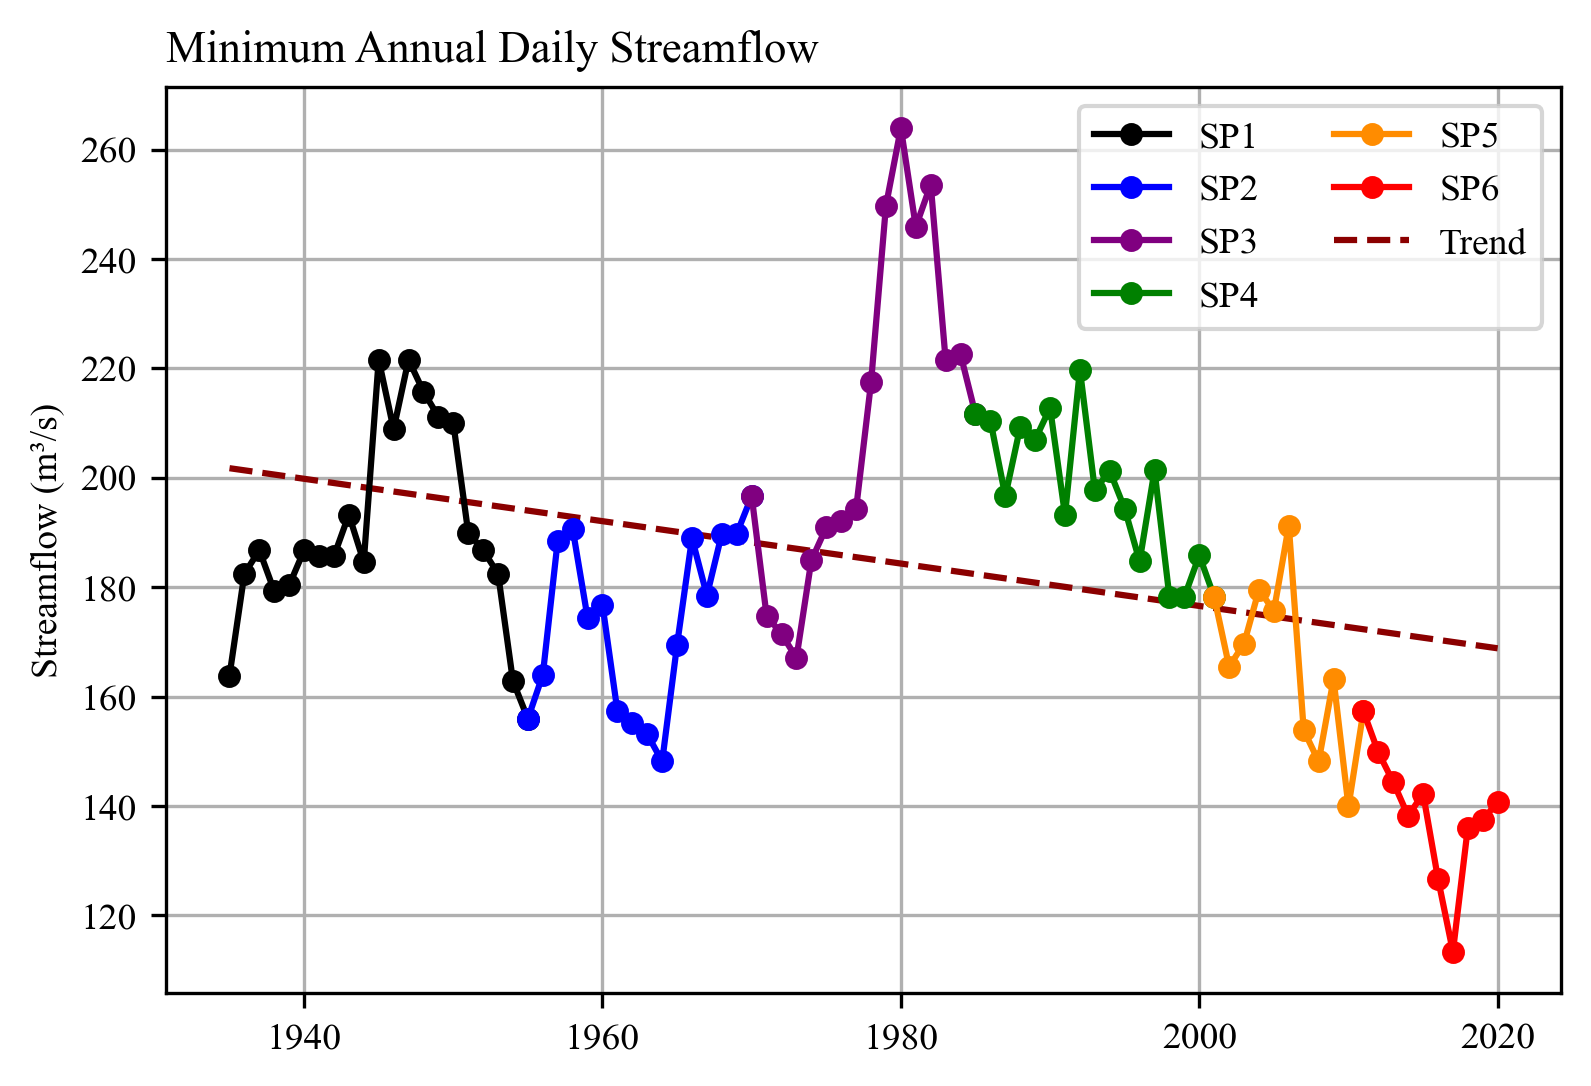
\includegraphics[scale = 1]{
                figs/Q_min_anual.png
                }
            \caption{
                Minimum Annual Daily Streamflow time series from 1935 to 2020. 
            }
            \label{fig:Q_min}
        \end{figure*}
        
        A marked interannual variability can be observed between the subperiods SP1 and SP3. In the subperiod SP3, a strong increasing behavior is noted, reaching the peak of the time series in 1980. 
        
        A predominantly decreasing behavior was observed between SP4 and SP6 periods, reaching the minimum of the time series in 2017. The behavior of these sub-periods attributes to this time series the decreasing trend evidenced by the MKS method.

        The Figure \ref{fig:FDC} and the Table \ref{tb:min_ref_flow} shows, respectively, the FDC curves and the adopted MRS ($Q_{95}$ and $Q_{7,10}$) for each subperiod highlighted in the Table \ref{tb:sub_periods_min_flow}. 

        \begin{figure*}
            \centering
                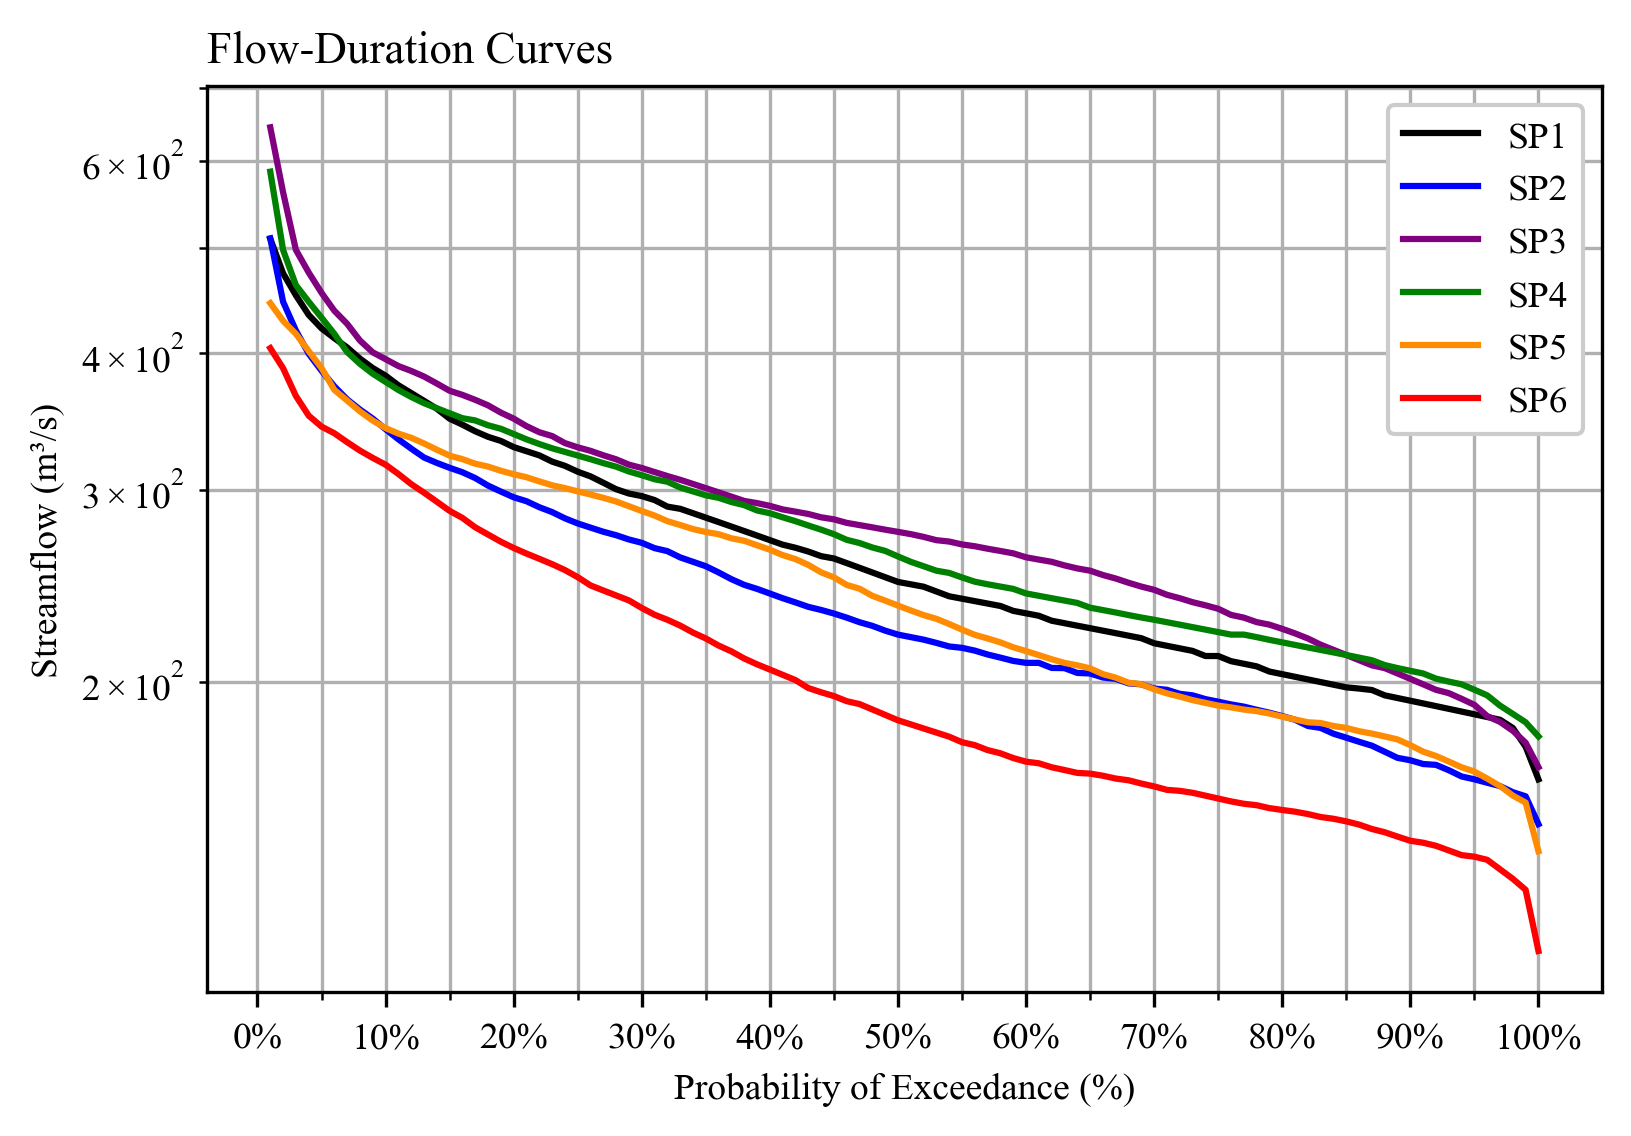
\includegraphics[scale = 1]{
                figs/Curvas_Permanencia.png
                }
            \caption{
                Flow-Duration Curves for each adopted subperiod (Table \ref{tb:sub_periods_min_flow})
            }
            \label{fig:FDC}
        \end{figure*}

        \begin{table}[width=.9\linewidth, cols=5]
            \caption{
            Minimum Reference Streamflows for each adopted subperiod
            }
            \label{tb:min_ref_flow}
            \begin{tabular*}{\tblwidth}{@{\extracolsep{\fill}} c c c}
            \toprule
                Subperiod & $Q_{95}\;(m^{3}/s)$ & $Q_{7,10}\;(m^{3}/s)$\\
            \midrule
                SP1 & 186.75 & 215.55 \\
                SP2 & 162.80 & 190.81 \\
                SP3 & 190.52 & 251.26 \\
                SP4 & 196.68 & 214.87 \\
                SP5 & 165.49 & 185.81 \\
                SP6 & 138.29 & 152.61 \\
            \bottomrule
            \end{tabular*}
        \end{table}

        The predominantly decreasing behavior of the minimum annual daily streamflow after SP3 produces successive reductions in FDC's streamflows in the SP4, SP5 and SP6 subperiods. The SP6 subperiod, according to its FDC, presented the lowest water availability of the entire evaluated period (1935-2020).

        The subperiods SP3 and SP4 show an interesting behavior in their FDC. The SP4's FDC shows the highest streamflow values for almost all exceedance probabilities, however, for large values ($\geq 80\%$), the streamflows of the SP4's FDC surpass of the SP3's FDC. According to the Figure \ref{fig:Q_min}, despite the peak value in SP3, this subperiod presented 8 of 15 years with minimum daily streamflows lower or of the same magnitude as those observed in SP4, which may justify the FDC's behavior above-mentioned.
        
        Regarding $Q_{95}$ , a significant variability in its value is observed between the SP1, SP2 and SP3 subperiods, from 186.75 $m^{3}/s$ to 162.80 $m^{3}/s$ and from 162.80 $m^{3}/s$ to 190.52 $m^{3}/s$. This behavior can be explained by the marked interannual variability of the annual minimum daily flow observed between these subperiods.

        In SP4 there is the highest value of $Q_{95}$  among the subperiods, 196.68 $m^{3}/s$, indicating the subperiod with the highest water availability. However, from this subperiod onwards, successive reductions are observed in the $Q_{95}$ values, reaching the lowest value in SP6: 138.29 $m^{3}/s$, a reduction of almost 30\%.

        Regarding $Q_{7,10}$, a similar behavior to that observed in $Q_{95}$ is noted, except for the occurrence of its highest value in SP3 instead of SP4. After the occurrence of this peak at SP3 (251.26 $m^{3}/s$), successive reductions are observed until reaching its minimum value at SP6 (152.61 $m^{3}/s$), a reduction of approximately 39\%.
        


        
